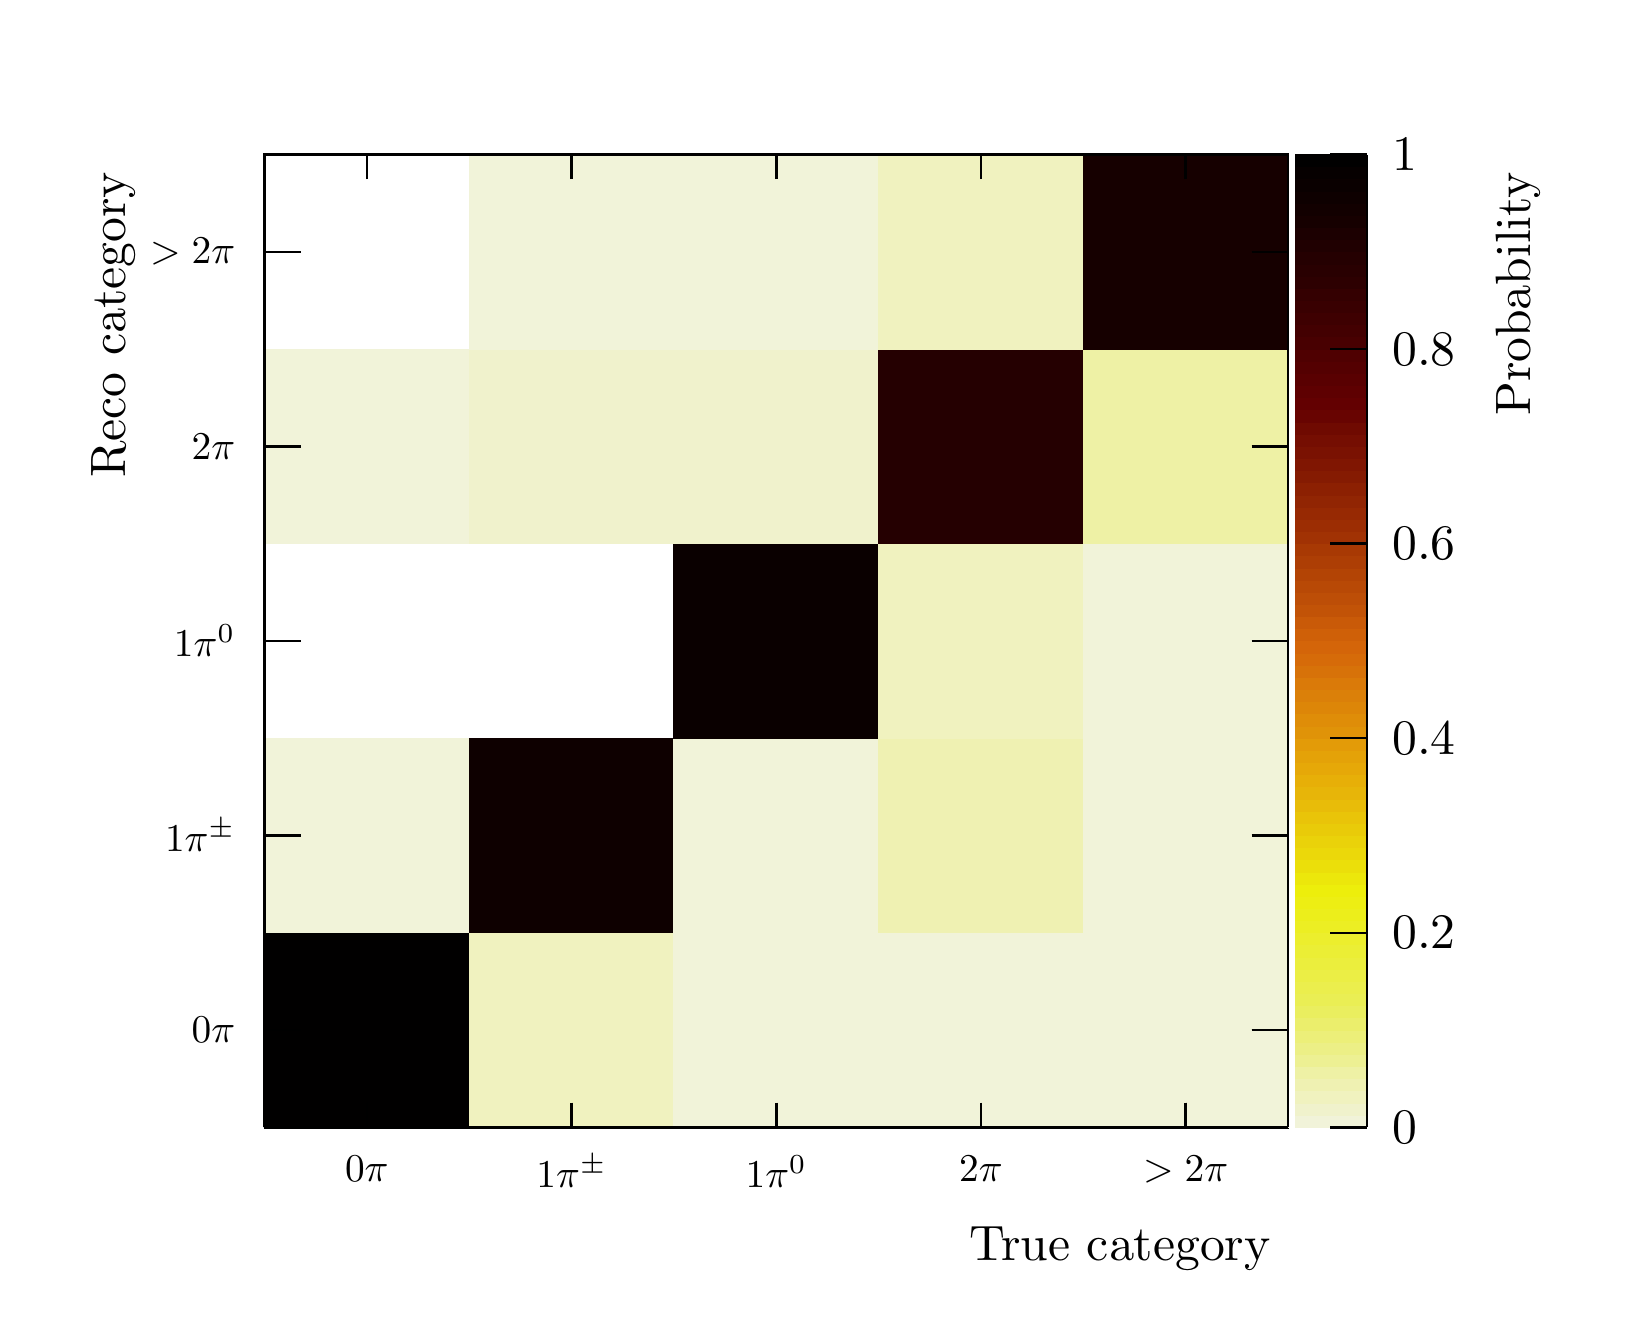
\begin{tikzpicture}
\pgfdeclareplotmark{cross} {
\pgfpathmoveto{\pgfpoint{-0.3\pgfplotmarksize}{\pgfplotmarksize}}
\pgfpathlineto{\pgfpoint{+0.3\pgfplotmarksize}{\pgfplotmarksize}}
\pgfpathlineto{\pgfpoint{+0.3\pgfplotmarksize}{0.3\pgfplotmarksize}}
\pgfpathlineto{\pgfpoint{+1\pgfplotmarksize}{0.3\pgfplotmarksize}}
\pgfpathlineto{\pgfpoint{+1\pgfplotmarksize}{-0.3\pgfplotmarksize}}
\pgfpathlineto{\pgfpoint{+0.3\pgfplotmarksize}{-0.3\pgfplotmarksize}}
\pgfpathlineto{\pgfpoint{+0.3\pgfplotmarksize}{-1.\pgfplotmarksize}}
\pgfpathlineto{\pgfpoint{-0.3\pgfplotmarksize}{-1.\pgfplotmarksize}}
\pgfpathlineto{\pgfpoint{-0.3\pgfplotmarksize}{-0.3\pgfplotmarksize}}
\pgfpathlineto{\pgfpoint{-1.\pgfplotmarksize}{-0.3\pgfplotmarksize}}
\pgfpathlineto{\pgfpoint{-1.\pgfplotmarksize}{0.3\pgfplotmarksize}}
\pgfpathlineto{\pgfpoint{-0.3\pgfplotmarksize}{0.3\pgfplotmarksize}}
\pgfpathclose
\pgfusepathqstroke
}
\pgfdeclareplotmark{cross*} {
\pgfpathmoveto{\pgfpoint{-0.3\pgfplotmarksize}{\pgfplotmarksize}}
\pgfpathlineto{\pgfpoint{+0.3\pgfplotmarksize}{\pgfplotmarksize}}
\pgfpathlineto{\pgfpoint{+0.3\pgfplotmarksize}{0.3\pgfplotmarksize}}
\pgfpathlineto{\pgfpoint{+1\pgfplotmarksize}{0.3\pgfplotmarksize}}
\pgfpathlineto{\pgfpoint{+1\pgfplotmarksize}{-0.3\pgfplotmarksize}}
\pgfpathlineto{\pgfpoint{+0.3\pgfplotmarksize}{-0.3\pgfplotmarksize}}
\pgfpathlineto{\pgfpoint{+0.3\pgfplotmarksize}{-1.\pgfplotmarksize}}
\pgfpathlineto{\pgfpoint{-0.3\pgfplotmarksize}{-1.\pgfplotmarksize}}
\pgfpathlineto{\pgfpoint{-0.3\pgfplotmarksize}{-0.3\pgfplotmarksize}}
\pgfpathlineto{\pgfpoint{-1.\pgfplotmarksize}{-0.3\pgfplotmarksize}}
\pgfpathlineto{\pgfpoint{-1.\pgfplotmarksize}{0.3\pgfplotmarksize}}
\pgfpathlineto{\pgfpoint{-0.3\pgfplotmarksize}{0.3\pgfplotmarksize}}
\pgfpathclose
\pgfusepathqfillstroke
}
\pgfdeclareplotmark{newstar} {
\pgfpathmoveto{\pgfqpoint{0pt}{\pgfplotmarksize}}
\pgfpathlineto{\pgfqpointpolar{44}{0.5\pgfplotmarksize}}
\pgfpathlineto{\pgfqpointpolar{18}{\pgfplotmarksize}}
\pgfpathlineto{\pgfqpointpolar{-20}{0.5\pgfplotmarksize}}
\pgfpathlineto{\pgfqpointpolar{-54}{\pgfplotmarksize}}
\pgfpathlineto{\pgfqpointpolar{-90}{0.5\pgfplotmarksize}}
\pgfpathlineto{\pgfqpointpolar{234}{\pgfplotmarksize}}
\pgfpathlineto{\pgfqpointpolar{198}{0.5\pgfplotmarksize}}
\pgfpathlineto{\pgfqpointpolar{162}{\pgfplotmarksize}}
\pgfpathlineto{\pgfqpointpolar{134}{0.5\pgfplotmarksize}}
\pgfpathclose
\pgfusepathqstroke
}
\pgfdeclareplotmark{newstar*} {
\pgfpathmoveto{\pgfqpoint{0pt}{\pgfplotmarksize}}
\pgfpathlineto{\pgfqpointpolar{44}{0.5\pgfplotmarksize}}
\pgfpathlineto{\pgfqpointpolar{18}{\pgfplotmarksize}}
\pgfpathlineto{\pgfqpointpolar{-20}{0.5\pgfplotmarksize}}
\pgfpathlineto{\pgfqpointpolar{-54}{\pgfplotmarksize}}
\pgfpathlineto{\pgfqpointpolar{-90}{0.5\pgfplotmarksize}}
\pgfpathlineto{\pgfqpointpolar{234}{\pgfplotmarksize}}
\pgfpathlineto{\pgfqpointpolar{198}{0.5\pgfplotmarksize}}
\pgfpathlineto{\pgfqpointpolar{162}{\pgfplotmarksize}}
\pgfpathlineto{\pgfqpointpolar{134}{0.5\pgfplotmarksize}}
\pgfpathclose
\pgfusepathqfillstroke
}
\definecolor{c}{rgb}{1,1,1};
\draw [color=c, fill=c] (0,0) rectangle (20,16.0446);
\draw [color=c, fill=c] (3,2.08579) rectangle (16,14.4401);
\definecolor{c}{rgb}{0,0,0};
\draw [c,line width=0.9] (3,2.08579) -- (3,14.4401) -- (16,14.4401) -- (16,2.08579) -- (3,2.08579);
\definecolor{c}{rgb}{1,1,1};
\draw [color=c, fill=c] (3,2.08579) rectangle (16,14.4401);
\definecolor{c}{rgb}{0,0,0};
\draw [c,line width=0.9] (3,2.08579) -- (3,14.4401) -- (16,14.4401) -- (16,2.08579) -- (3,2.08579);
\definecolor{c}{rgb}{0.00551471,0,0.000122549};
\draw [color=c, fill=c] (3,2.08579) rectangle (5.6,4.55666);
\definecolor{c}{rgb}{0.939911,0.947249,0.748261};
\draw [color=c, fill=c] (5.6,2.08579) rectangle (8.2,4.55666);
\definecolor{c}{rgb}{0.945984,0.951044,0.850727};
\draw [color=c, fill=c] (8.2,2.08579) rectangle (10.8,4.55666);
\draw [color=c, fill=c] (10.8,2.08579) rectangle (13.4,4.55666);
\draw [color=c, fill=c] (13.4,2.08579) rectangle (16,4.55666);
\draw [color=c, fill=c] (3,4.55666) rectangle (5.6,7.02752);
\definecolor{c}{rgb}{0.0551471,0,0.00122549};
\draw [color=c, fill=c] (5.6,4.55666) rectangle (8.2,7.02752);
\definecolor{c}{rgb}{0.945984,0.951044,0.850727};
\draw [color=c, fill=c] (8.2,4.55666) rectangle (10.8,7.02752);
\definecolor{c}{rgb}{0.936875,0.945351,0.697027};
\draw [color=c, fill=c] (10.8,4.55666) rectangle (13.4,7.02752);
\definecolor{c}{rgb}{0.945984,0.951044,0.850727};
\draw [color=c, fill=c] (13.4,4.55666) rectangle (16,7.02752);
\definecolor{c}{rgb}{0.0386029,0,0.000857843};
\draw [color=c, fill=c] (8.2,7.02752) rectangle (10.8,9.49838);
\definecolor{c}{rgb}{0.939911,0.947249,0.748261};
\draw [color=c, fill=c] (10.8,7.02752) rectangle (13.4,9.49838);
\definecolor{c}{rgb}{0.945984,0.951044,0.850727};
\draw [color=c, fill=c] (13.4,7.02752) rectangle (16,9.49838);
\draw [color=c, fill=c] (3,9.49838) rectangle (5.6,11.9692);
\definecolor{c}{rgb}{0.942948,0.949146,0.799494};
\draw [color=c, fill=c] (5.6,9.49838) rectangle (8.2,11.9692);
\draw [color=c, fill=c] (8.2,9.49838) rectangle (10.8,11.9692);
\definecolor{c}{rgb}{0.143382,0,0.00318627};
\draw [color=c, fill=c] (10.8,9.49838) rectangle (13.4,11.9692);
\definecolor{c}{rgb}{0.933839,0.943453,0.645794};
\draw [color=c, fill=c] (13.4,9.49838) rectangle (16,11.9692);
\definecolor{c}{rgb}{0.945984,0.951044,0.850727};
\draw [color=c, fill=c] (5.6,11.9692) rectangle (8.2,14.4401);
\draw [color=c, fill=c] (8.2,11.9692) rectangle (10.8,14.4401);
\definecolor{c}{rgb}{0.939911,0.947249,0.748261};
\draw [color=c, fill=c] (10.8,11.9692) rectangle (13.4,14.4401);
\definecolor{c}{rgb}{0.0882353,0,0.00196078};
\draw [color=c, fill=c] (13.4,11.9692) rectangle (16,14.4401);
\definecolor{c}{rgb}{0,0,0};
\draw [c,line width=0.9] (3,2.08579) -- (16,2.08579);
\draw [anchor=north] (4.3,1.90048) node[scale=1.42291, color=c, rotate=0]{$0\pi$};
\draw [anchor=north] (6.9,1.90048) node[scale=1.42291, color=c, rotate=0]{$1\pi^{\pm}$};
\draw [anchor=north] (9.5,1.90048) node[scale=1.42291, color=c, rotate=0]{$1\pi^{0}$};
\draw [anchor=north] (12.1,1.90048) node[scale=1.42291, color=c, rotate=0]{$2\pi$};
\draw [anchor=north] (14.7,1.90048) node[scale=1.42291, color=c, rotate=0]{$>2\pi$};
\draw [c,line width=0.9] (4.3,2.39866) -- (4.3,2.08579);
\draw [c,line width=0.9] (6.9,2.39866) -- (6.9,2.08579);
\draw [c,line width=0.9] (9.5,2.39866) -- (9.5,2.08579);
\draw [c,line width=0.9] (12.1,2.39866) -- (12.1,2.08579);
\draw [c,line width=0.9] (14.7,2.39866) -- (14.7,2.08579);
\draw [c,line width=0.9] (4.3,2.39866) -- (4.3,2.08579);
\draw [c,line width=0.9] (14.7,2.39866) -- (14.7,2.08579);
\draw [anchor= east] (16,0.545515) node[scale=1.7941, color=c, rotate=0]{ True category};
\draw [c,line width=0.9] (3,14.4401) -- (16,14.4401);
\draw [c,line width=0.9] (4.3,14.1272) -- (4.3,14.4401);
\draw [c,line width=0.9] (6.9,14.1272) -- (6.9,14.4401);
\draw [c,line width=0.9] (9.5,14.1272) -- (9.5,14.4401);
\draw [c,line width=0.9] (12.1,14.1272) -- (12.1,14.4401);
\draw [c,line width=0.9] (14.7,14.1272) -- (14.7,14.4401);
\draw [c,line width=0.9] (4.3,14.1272) -- (4.3,14.4401);
\draw [c,line width=0.9] (14.7,14.1272) -- (14.7,14.4401);
\draw [c,line width=0.9] (3,2.08579) -- (3,14.4401);
\draw [anchor= east] (2.805,3.32123) node[scale=1.42291, color=c, rotate=0]{$0\pi$};
\draw [anchor= east] (2.805,5.79209) node[scale=1.42291, color=c, rotate=0]{$1\pi^{\pm}$};
\draw [anchor= east] (2.805,8.26295) node[scale=1.42291, color=c, rotate=0]{$1\pi^{0}$};
\draw [anchor= east] (2.805,10.7338) node[scale=1.42291, color=c, rotate=0]{$2\pi$};
\draw [anchor= east] (2.805,13.2047) node[scale=1.42291, color=c, rotate=0]{$>2\pi$};
\draw [c,line width=0.9] (3.462,3.32123) -- (3,3.32123);
\draw [c,line width=0.9] (3.462,5.79209) -- (3,5.79209);
\draw [c,line width=0.9] (3.462,8.26295) -- (3,8.26295);
\draw [c,line width=0.9] (3.462,10.7338) -- (3,10.7338);
\draw [c,line width=0.9] (3.462,13.2047) -- (3,13.2047);
\draw [c,line width=0.9] (3.462,3.32123) -- (3,3.32123);
\draw [c,line width=0.9] (3.462,13.2047) -- (3,13.2047);
\draw [anchor= east] (1.08,14.4401) node[scale=1.7941, color=c, rotate=90]{ Reco category};
\draw [c,line width=0.9] (16,2.08579) -- (16,14.4401);
\draw [c,line width=0.9] (15.538,3.32123) -- (16,3.32123);
\draw [c,line width=0.9] (15.538,5.79209) -- (16,5.79209);
\draw [c,line width=0.9] (15.538,8.26295) -- (16,8.26295);
\draw [c,line width=0.9] (15.538,10.7338) -- (16,10.7338);
\draw [c,line width=0.9] (15.538,13.2047) -- (16,13.2047);
\draw [c,line width=0.9] (15.538,3.32123) -- (16,3.32123);
\draw [c,line width=0.9] (15.538,13.2047) -- (16,13.2047);
\definecolor{c}{rgb}{0.945984,0.951044,0.850727};
\draw [color=c, fill=c] (16.1,2.08579) rectangle (17,2.24022);
\definecolor{c}{rgb}{0.942948,0.949146,0.799494};
\draw [color=c, fill=c] (16.1,2.24022) rectangle (17,2.39465);
\definecolor{c}{rgb}{0.939911,0.947249,0.748261};
\draw [color=c, fill=c] (16.1,2.39465) rectangle (17,2.54908);
\definecolor{c}{rgb}{0.936875,0.945351,0.697027};
\draw [color=c, fill=c] (16.1,2.54908) rectangle (17,2.70351);
\definecolor{c}{rgb}{0.933839,0.943453,0.645794};
\draw [color=c, fill=c] (16.1,2.70351) rectangle (17,2.85794);
\definecolor{c}{rgb}{0.929791,0.940923,0.577483};
\draw [color=c, fill=c] (16.1,2.85794) rectangle (17,3.01237);
\definecolor{c}{rgb}{0.926755,0.939026,0.526249};
\draw [color=c, fill=c] (16.1,3.01237) rectangle (17,3.1668);
\definecolor{c}{rgb}{0.923719,0.937128,0.475016};
\draw [color=c, fill=c] (16.1,3.1668) rectangle (17,3.32123);
\definecolor{c}{rgb}{0.920683,0.935231,0.423782};
\draw [color=c, fill=c] (16.1,3.32123) rectangle (17,3.47565);
\definecolor{c}{rgb}{0.917647,0.933333,0.372549};
\draw [color=c, fill=c] (16.1,3.47565) rectangle (17,3.63008);
\definecolor{c}{rgb}{0.919118,0.933333,0.331373};
\draw [color=c, fill=c] (16.1,3.63008) rectangle (17,3.78451);
\definecolor{c}{rgb}{0.920221,0.933333,0.30049};
\draw [color=c, fill=c] (16.1,3.78451) rectangle (17,3.93894);
\definecolor{c}{rgb}{0.921324,0.933333,0.269608};
\draw [color=c, fill=c] (16.1,3.93894) rectangle (17,4.09337);
\definecolor{c}{rgb}{0.922426,0.933333,0.238725};
\draw [color=c, fill=c] (16.1,4.09337) rectangle (17,4.2478);
\definecolor{c}{rgb}{0.923529,0.933333,0.207843};
\draw [color=c, fill=c] (16.1,4.2478) rectangle (17,4.40223);
\definecolor{c}{rgb}{0.924632,0.933333,0.176961};
\draw [color=c, fill=c] (16.1,4.40223) rectangle (17,4.55666);
\definecolor{c}{rgb}{0.926103,0.933333,0.135784};
\draw [color=c, fill=c] (16.1,4.55666) rectangle (17,4.71109);
\definecolor{c}{rgb}{0.927206,0.933333,0.104902};
\draw [color=c, fill=c] (16.1,4.71109) rectangle (17,4.86552);
\definecolor{c}{rgb}{0.928309,0.933333,0.0740196};
\draw [color=c, fill=c] (16.1,4.86552) rectangle (17,5.01994);
\definecolor{c}{rgb}{0.929412,0.933333,0.0431373};
\draw [color=c, fill=c] (16.1,5.01994) rectangle (17,5.17437);
\definecolor{c}{rgb}{0.926838,0.907598,0.0420343};
\draw [color=c, fill=c] (16.1,5.17437) rectangle (17,5.3288);
\definecolor{c}{rgb}{0.923407,0.873284,0.0405637};
\draw [color=c, fill=c] (16.1,5.3288) rectangle (17,5.48323);
\definecolor{c}{rgb}{0.920833,0.847549,0.0394608};
\draw [color=c, fill=c] (16.1,5.48323) rectangle (17,5.63766);
\definecolor{c}{rgb}{0.91826,0.821814,0.0383578};
\draw [color=c, fill=c] (16.1,5.63766) rectangle (17,5.79209);
\definecolor{c}{rgb}{0.915686,0.796078,0.0372549};
\draw [color=c, fill=c] (16.1,5.79209) rectangle (17,5.94652);
\definecolor{c}{rgb}{0.913113,0.770343,0.036152};
\draw [color=c, fill=c] (16.1,5.94652) rectangle (17,6.10095);
\definecolor{c}{rgb}{0.909681,0.736029,0.0346814};
\draw [color=c, fill=c] (16.1,6.10095) rectangle (17,6.25538);
\definecolor{c}{rgb}{0.907108,0.710294,0.0335784};
\draw [color=c, fill=c] (16.1,6.25538) rectangle (17,6.40981);
\definecolor{c}{rgb}{0.904534,0.684559,0.0324755};
\draw [color=c, fill=c] (16.1,6.40981) rectangle (17,6.56423);
\definecolor{c}{rgb}{0.901961,0.658824,0.0313726};
\draw [color=c, fill=c] (16.1,6.56423) rectangle (17,6.71866);
\definecolor{c}{rgb}{0.895343,0.634191,0.0317402};
\draw [color=c, fill=c] (16.1,6.71866) rectangle (17,6.87309);
\definecolor{c}{rgb}{0.888726,0.609559,0.0321078};
\draw [color=c, fill=c] (16.1,6.87309) rectangle (17,7.02752);
\definecolor{c}{rgb}{0.879902,0.576716,0.032598};
\draw [color=c, fill=c] (16.1,7.02752) rectangle (17,7.18195);
\definecolor{c}{rgb}{0.873284,0.552083,0.0329657};
\draw [color=c, fill=c] (16.1,7.18195) rectangle (17,7.33638);
\definecolor{c}{rgb}{0.866667,0.527451,0.0333333};
\draw [color=c, fill=c] (16.1,7.33638) rectangle (17,7.49081);
\definecolor{c}{rgb}{0.860049,0.502819,0.033701};
\draw [color=c, fill=c] (16.1,7.49081) rectangle (17,7.64524);
\definecolor{c}{rgb}{0.853431,0.478186,0.0340686};
\draw [color=c, fill=c] (16.1,7.64524) rectangle (17,7.79967);
\definecolor{c}{rgb}{0.844608,0.445343,0.0345588};
\draw [color=c, fill=c] (16.1,7.79967) rectangle (17,7.95409);
\definecolor{c}{rgb}{0.83799,0.420711,0.0349265};
\draw [color=c, fill=c] (16.1,7.95409) rectangle (17,8.10852);
\definecolor{c}{rgb}{0.831373,0.396078,0.0352941};
\draw [color=c, fill=c] (16.1,8.10852) rectangle (17,8.26295);
\definecolor{c}{rgb}{0.810784,0.37549,0.0330882};
\draw [color=c, fill=c] (16.1,8.26295) rectangle (17,8.41738);
\definecolor{c}{rgb}{0.790196,0.354902,0.0308824};
\draw [color=c, fill=c] (16.1,8.41738) rectangle (17,8.57181);
\definecolor{c}{rgb}{0.762745,0.327451,0.0279412};
\draw [color=c, fill=c] (16.1,8.57181) rectangle (17,8.72624);
\definecolor{c}{rgb}{0.742157,0.306863,0.0257353};
\draw [color=c, fill=c] (16.1,8.72624) rectangle (17,8.88067);
\definecolor{c}{rgb}{0.721569,0.286275,0.0235294};
\draw [color=c, fill=c] (16.1,8.88067) rectangle (17,9.0351);
\definecolor{c}{rgb}{0.70098,0.265686,0.0213235};
\draw [color=c, fill=c] (16.1,9.0351) rectangle (17,9.18953);
\definecolor{c}{rgb}{0.680392,0.245098,0.0191176};
\draw [color=c, fill=c] (16.1,9.18953) rectangle (17,9.34396);
\definecolor{c}{rgb}{0.659804,0.22451,0.0169118};
\draw [color=c, fill=c] (16.1,9.34396) rectangle (17,9.49838);
\definecolor{c}{rgb}{0.632353,0.197059,0.0139706};
\draw [color=c, fill=c] (16.1,9.49838) rectangle (17,9.65281);
\definecolor{c}{rgb}{0.611765,0.176471,0.0117647};
\draw [color=c, fill=c] (16.1,9.65281) rectangle (17,9.80724);
\definecolor{c}{rgb}{0.590809,0.159926,0.0110294};
\draw [color=c, fill=c] (16.1,9.80724) rectangle (17,9.96167);
\definecolor{c}{rgb}{0.569853,0.143382,0.0102941};
\draw [color=c, fill=c] (16.1,9.96167) rectangle (17,10.1161);
\definecolor{c}{rgb}{0.548897,0.126838,0.00955882};
\draw [color=c, fill=c] (16.1,10.1161) rectangle (17,10.2705);
\definecolor{c}{rgb}{0.520956,0.104779,0.00857843};
\draw [color=c, fill=c] (16.1,10.2705) rectangle (17,10.425);
\definecolor{c}{rgb}{0.5,0.0882353,0.00784314};
\draw [color=c, fill=c] (16.1,10.425) rectangle (17,10.5794);
\definecolor{c}{rgb}{0.479044,0.0716912,0.00710784};
\draw [color=c, fill=c] (16.1,10.5794) rectangle (17,10.7338);
\definecolor{c}{rgb}{0.458088,0.0551471,0.00637255};
\draw [color=c, fill=c] (16.1,10.7338) rectangle (17,10.8882);
\definecolor{c}{rgb}{0.437132,0.0386029,0.00563726};
\draw [color=c, fill=c] (16.1,10.8882) rectangle (17,11.0427);
\definecolor{c}{rgb}{0.409191,0.0165441,0.00465686};
\draw [color=c, fill=c] (16.1,11.0427) rectangle (17,11.1971);
\definecolor{c}{rgb}{0.388235,0,0.00392157};
\draw [color=c, fill=c] (16.1,11.1971) rectangle (17,11.3515);
\definecolor{c}{rgb}{0.368382,0,0.00392157};
\draw [color=c, fill=c] (16.1,11.3515) rectangle (17,11.506);
\definecolor{c}{rgb}{0.348529,0,0.00392157};
\draw [color=c, fill=c] (16.1,11.506) rectangle (17,11.6604);
\definecolor{c}{rgb}{0.328676,0,0.00392157};
\draw [color=c, fill=c] (16.1,11.6604) rectangle (17,11.8148);
\definecolor{c}{rgb}{0.308824,0,0.00392157};
\draw [color=c, fill=c] (16.1,11.8148) rectangle (17,11.9692);
\definecolor{c}{rgb}{0.282353,0,0.00392157};
\draw [color=c, fill=c] (16.1,11.9692) rectangle (17,12.1237);
\definecolor{c}{rgb}{0.2625,0,0.00392157};
\draw [color=c, fill=c] (16.1,12.1237) rectangle (17,12.2781);
\definecolor{c}{rgb}{0.242647,0,0.00392157};
\draw [color=c, fill=c] (16.1,12.2781) rectangle (17,12.4325);
\definecolor{c}{rgb}{0.222794,0,0.00392157};
\draw [color=c, fill=c] (16.1,12.4325) rectangle (17,12.587);
\definecolor{c}{rgb}{0.202941,0,0.00392157};
\draw [color=c, fill=c] (16.1,12.587) rectangle (17,12.7414);
\definecolor{c}{rgb}{0.176471,0,0.00392157};
\draw [color=c, fill=c] (16.1,12.7414) rectangle (17,12.8958);
\definecolor{c}{rgb}{0.159926,0,0.00355392};
\draw [color=c, fill=c] (16.1,12.8958) rectangle (17,13.0503);
\definecolor{c}{rgb}{0.143382,0,0.00318627};
\draw [color=c, fill=c] (16.1,13.0503) rectangle (17,13.2047);
\definecolor{c}{rgb}{0.126838,0,0.00281863};
\draw [color=c, fill=c] (16.1,13.2047) rectangle (17,13.3591);
\definecolor{c}{rgb}{0.110294,0,0.00245098};
\draw [color=c, fill=c] (16.1,13.3591) rectangle (17,13.5135);
\definecolor{c}{rgb}{0.0882353,0,0.00196078};
\draw [color=c, fill=c] (16.1,13.5135) rectangle (17,13.668);
\definecolor{c}{rgb}{0.0716912,0,0.00159314};
\draw [color=c, fill=c] (16.1,13.668) rectangle (17,13.8224);
\definecolor{c}{rgb}{0.0551471,0,0.00122549};
\draw [color=c, fill=c] (16.1,13.8224) rectangle (17,13.9768);
\definecolor{c}{rgb}{0.0386029,0,0.000857843};
\draw [color=c, fill=c] (16.1,13.9768) rectangle (17,14.1313);
\definecolor{c}{rgb}{0.0220588,0,0.000490196};
\draw [color=c, fill=c] (16.1,14.1313) rectangle (17,14.2857);
\definecolor{c}{rgb}{0.00551471,0,0.000122549};
\draw [color=c, fill=c] (16.1,14.2857) rectangle (17,14.4401);
\definecolor{c}{rgb}{0,0,0};
\draw [c,line width=0.9] (17,2.08579) -- (17,14.4401);
\draw [c,line width=0.9] (16.538,2.08579) -- (17,2.08579);
\draw [c,line width=0.9] (16.538,4.55666) -- (17,4.55666);
\draw [c,line width=0.9] (16.538,7.02752) -- (17,7.02752);
\draw [c,line width=0.9] (16.538,9.49838) -- (17,9.49838);
\draw [c,line width=0.9] (16.538,11.9692) -- (17,11.9692);
\draw [c,line width=0.9] (16.538,14.4401) -- (17,14.4401);
\draw [c,line width=0.9] (16.538,14.4401) -- (17,14.4401);
\draw [anchor= west] (17.1,2.08579) node[scale=1.7941, color=c, rotate=0]{0};
\draw [anchor= west] (17.1,4.55666) node[scale=1.7941, color=c, rotate=0]{0.2};
\draw [anchor= west] (17.1,7.02752) node[scale=1.7941, color=c, rotate=0]{0.4};
\draw [anchor= west] (17.1,9.49838) node[scale=1.7941, color=c, rotate=0]{0.6};
\draw [anchor= west] (17.1,11.9692) node[scale=1.7941, color=c, rotate=0]{0.8};
\draw [anchor= west] (17.1,14.4401) node[scale=1.7941, color=c, rotate=0]{1};
\draw [anchor= east] (18.92,14.4401) node[scale=1.7941, color=c, rotate=90]{ Probability};
\definecolor{c}{rgb}{1,1,1};
\draw [color=c, fill=c] (2,15.0819) rectangle (18,15.9643);
\definecolor{c}{rgb}{0,0,0};
%\draw (10,15.5231) node[scale=1.67037, color=c, rotate=0]{Final state confusion matrix in HPgTPC};
\end{tikzpicture}
